\documentclass[12pt,a4paper]{article}
\usepackage{cmap} % Makes the PDF copiable. See http://tex.stackexchange.com/a/64198/25761
\usepackage[T1]{fontenc}
\usepackage[brazil]{babel}
\usepackage[utf8]{inputenc}
\usepackage{amsmath}
\usepackage{amsfonts}
\usepackage{amssymb}
\usepackage{amsthm}
\usepackage{textcomp} % \degree
\usepackage{gensymb} % \degree
\usepackage[usenames,svgnames,dvipsnames]{xcolor}
\usepackage{hyperref}
\usepackage{multicol}
\usepackage{graphicx}
\usepackage[margin=2cm]{geometry}
\usepackage{systeme}

\hypersetup{
    colorlinks = true,
    allcolors = {blue}
}

% TODO: Consider using exsheets
% http://linorg.usp.br/CTAN/macros/latex/contrib/exsheets/exsheets_en.pdf
%
% http://ctan.org/tex-archive/macros/latex/contrib/exercise/
% Options: answerdelayed,lastexercise,noanswer
\usepackage[answerdelayed,lastexercise]{exercise}

\addto\captionsbrazil{%
\def\listexercisename{Lista de exerc\'icios}%
\def\ExerciseName{Exerc\'icio}%
\def\AnswerName{Solu\c{c}\~ao do exerc\'icio}%
\def\ExerciseListName{Ex.}%
\def\AnswerListName{Solu\c{c}\~ao}%
\def\ExePartName{Parte}%
\def\ArticleOf{de\ }%
}

\renewcommand{\ExerciseHeaderTitle}{(\ExerciseTitle)\ }
\renewcommand{\ExerciseListHeader}{%\ExerciseHeaderDifficulty%
\textbf{%\ExerciseListName\
\ExerciseHeaderNB.\ %
%\ --- \
\ExerciseHeaderTitle}%
%\ExerciseHeaderOrigin
\ignorespaces}
\renewcommand{\AnswerListHeader}{\textbf{\ExerciseHeaderNB.\ (\AnswerListName)\ }}

\newcommand*\im[1]{\operatorname{Im}\left(#1\right)}
\newcommand*\R{\mathbb{R}}

% Loop Space / CC BY-SA-3.0 / https://tex.stackexchange.com/a/2238/25761
\newenvironment{amatrix}[1]{%
  \left[\begin{array}{@{}*{#1}{c}|c@{}}
}{%
  \end{array}\right]
}

% Loop Space / CC BY-SA-3.0 / https://tex.stackexchange.com/a/3164/25761
%--------grstep
% For denoting a Gauss' reduction step.
% Use as: \grstep{\rho_1+\rho_3} or \grstep[2\rho_5 \\ 3\rho_6]{\rho_1+\rho_3}
\newcommand{\grstep}[2][\relax]{%
   \ensuremath{\mathrel{
       {\mathop{\longrightarrow}\limits^{#2\mathstrut}_{
                                     \begin{subarray}{l} #1 \end{subarray}}}}}}

\renewcommand{\theenumi}{\alph{enumi}}
\renewcommand\labelenumi{(\theenumi) }

\newcommand*\tipo{Prova III}
\newcommand*\turma{NEX162-C}
\newcommand*\disciplina{ALI0001}
\newcommand*\eu{Helder G. G. de Lima}
\newcommand*\data{04/11/2016}

\author{\eu}
\title{\tipo - \disciplina}
\date{\data}

\begin{document}
\thispagestyle{empty}
\newgeometry{margin=2cm,bottom=0.5cm}
\begin{center}

\includegraphics[width=9.0cm]{marca} \\
\textbf{\tipo\ (\disciplina / \turma)} \\
Prof. \eu\footnote{
Este é um material de acesso livre distribuído sob os termos da licença \href{https://creativecommons.org/licenses/by-sa/4.0/deed.pt_BR}{Creative Commons BY-SA 4.0}}
\end{center}

\noindent Nome do(a) aluno(a): \underline{\hspace{9,7cm}} Data: \underline{\data}

%\section*{Instruções}
\begin{center}\fbox{
\begin{minipage}{14cm}

{\footnotesize
\begin{itemize}
\renewcommand{\theenumi}{\Roman{enumi}}
\item Identifique-se em todas as folhas.
\item Mantenha o celular e os demais equipamentos eletrônicos desligados durante a prova.
\item Escolha os itens a resolver de modo a totalizar até 10,0 pontos.
\end{itemize}
}

\end{minipage}
}
\end{center}

%\section*{Questões}
\begin{ExerciseList}

\Exercise%[title={2,0}]
Seja $L_1: M_2 \to M_2$ a função definida por $L_1(X) = 2X - X^T$.
\begin{enumerate}
\item \textbf{(1,0)} Mostre que $L_1$ é uma transformação linear.
\item \textbf{(1,0)} Obtenha as dimensões do núcleo e da imagem de $L_1$.
\item \textbf{(1,0)} A transformação $L_1$ é injetora? E sobrejetora? Justifique suas respostas.
\item \textbf{(1,0)} Se $L_2:M_2 \to M_2$ é a transformação linear definida por $L_2(X) = \frac{2}{3}X +\frac{1}{3}X^T$, obtenha a composta $(L_2 \circ L_1)(X)$ e a matriz de $L_2 \circ L_1$ em relação à base canônica de $M_2$.
\end{enumerate}
\Answer
\begin{enumerate}
\item Uma das condições para $L_1$ ser considerada linear é que ela preserve a soma de vetores. Pelas propriedades das operações matriciais, tem-se para quaisquer $A,B \in M_2$:
\begin{align*}
L_1(A+B)
& = 2(A+B) - (A+B)^T
= 2A+2B - (A^T+B^T) \\
& = (2A-A^T) + (2B - B^T)
= L_1(A) + L_1(B).
\end{align*}
A outra condição é que $L_1$ preserve a multiplicação por escalar. Dado $k \in \R$ e $A \in M_2$, tem-se:
\begin{align*}
L_1(kA)
= 2(kA) - (kA)^T
= k(2A) - k(A^T)
= k(2A - A^T)
= kL_1(A).
\end{align*}
Como $L_1$ satisfaz ambas as exigências, $L_1$ é uma transformação linear.

\item Como $L_1\left( \begin{bmatrix}
a & b \\ c & d
\end{bmatrix} \right)
=
2 \begin{bmatrix}
a & b \\ c & d
\end{bmatrix}
-
\begin{bmatrix}
a & c \\ b & d
\end{bmatrix}
=
\begin{bmatrix}
a & 2b-c \\ 2c-b & d
\end{bmatrix}$, tem-se para $X = \begin{bmatrix}
a & b \\ c & d
\end{bmatrix}$ que

\[
X \in N(L_1)
\Leftrightarrow
\begin{bmatrix}
a & 2b-c \\ 2c-b & d
\end{bmatrix}
=
\begin{bmatrix}
0 & 0 \\ 0 & 0
\end{bmatrix}
\Leftrightarrow
\begin{cases}
a&=0\\
2b-c&=0\\
2c-b&=0\\
d&=0
\end{cases}
\Leftrightarrow
\begin{cases}
a=0\\
b=0\\
c=0\\
d=0
\end{cases}
\Leftrightarrow
X = \begin{bmatrix}
0 & 0 \\ 0 & 0
\end{bmatrix}
\]
Assim, $N(L_1) = \left\{ \begin{bmatrix}
0 & 0 \\ 0 & 0
\end{bmatrix} \right\}$ e $\dim{ N(L_1) } = 0$. Como $\dim{ N(L_1) } + \dim{ \im{L_1} } = \dim{ M_2 }$, resulta que $\dim{ \im{L_1} } = 4$.

\item Pelo item anterior, $\dim{ N(L_1) } = 0$, então $L_1$ é injetora. Mas o domínio e o contradomínio de $L_1$ têm a mesma dimensão, então $L_1$ também é sobrejetora (isto é, $\im{L_1} = M_2$).

\item Sendo $L_2(X) = \frac{2}{3}X +\frac{1}{3}X^T = \frac{1}{3}(2X + X^T)$, tem-se para todo $X = \begin{bmatrix}
a & b \\ c & d
\end{bmatrix} \in M_2$:
\begin{align*}
(L_2 \circ L_1)(X)
& = L_2 ( L_1(X) )
= L_2 \left( \begin{bmatrix}
a & 2b-c \\ 2c-b & d
\end{bmatrix} \right) \\
& = \frac{1}{3}
\left( 2\begin{bmatrix}
a & 2b-c \\ 2c-b & d
\end{bmatrix} + \begin{bmatrix}
a & 2c-b \\ 2b-c & d
\end{bmatrix} \right) \\
& = \frac{1}{3} \begin{bmatrix}
2a + a & 2(2b-c) + (2c-b) \\ 2(2c-b)+(2b-c) & 2d + d
\end{bmatrix}
= \begin{bmatrix}
a & b \\ c & d
\end{bmatrix}.
\end{align*}

\textbf{Solução alternativa}: usando as propriedades das operações com matrizes, obtém-se
$(L_2 \circ L_1)(X)
= L_2( L_1(X) )
= L_2(2X - X^T)
= \frac{2}{3}(2X - X^T) +\frac{1}{3}(2X - X^T)^T
= \frac{4}{3}X - \frac{2}{3}X^T +\frac{2}{3}X^T - \frac{1}{3}X
= X$.

Resulta, de todo modo, que $(L_2 \circ L_1) (X) = X$, $\forall X \in M_2$, ou seja, $L_2 \circ L_1$ é o operador identidade em $M_2$. Em particular, se $C = \{ e_{11}, e_{12}, e_{21}, e_{22} \}$ é a base canônica de $M_2$, então $(L_2 \circ L_1) (e_{ij}) = e_{ij}$ e a matriz de $L_2 \circ L_1$ nesta base é a matriz identidade $4 \times 4$:
\[
[L_2 \circ L_1] = \begin{bmatrix}
1 & 0 & 0 & 0\\
0 & 1 & 0 & 0\\
0 & 0 & 1 & 0\\
0 & 0 & 0 & 1
\end{bmatrix} = I_{4}.
\]
\end{enumerate}

\Exercise%[title={2,0}]
Seja $T: P_1 \to P_2$ uma transformação linear.
\begin{enumerate}
\item \textbf{(2,0)} Supondo que $T(2x+1) = x^2+x$ e $T(4x)= 2x^2$, obtenha a fórmula para $T(ax + b)$.
\item \textbf{(2,0)} Obtenha a matriz $[T]^\alpha_\beta$ de $T$ em relação às bases $\alpha = \{1, x\}$ e $\beta = \{1, x, x^2\}$.
\end{enumerate}
\Answer
\begin{enumerate}
\item Como os vetores $v_1 = 2x+1$ e $v_2 = 4x$ não são múltiplos um do outro, $B = \{v_1,v_2\}$ é linearmente independente e gera $P_1$, pois $\dim{P_1} = 2$. Logo, é possível escrever qualquer $p(x) = ax + b \in P_1$ como combinação linear de $v_1$ e $v_2$:
\[
ax + b
= \alpha(2x+1) + \beta(4x)
= (2\alpha + 4\beta)x + (\alpha)1
\Leftrightarrow
\begin{cases}
2\alpha + 4\beta &= a\\
\alpha &= b
\end{cases}
\Leftrightarrow
\begin{cases}
\alpha &= b\\
\beta  &= \frac{a-2b}{4}
\end{cases}
\]

Assim, $ax+b = b(2x+1) + \frac{a-2b}{4}(4x)$ e pode-se usar a linearidade da função $T$ para obter:
\[
T(ax+b)
= bT(2x+1) + \frac{a-2b}{4}T(4x)
= b(x^2+x) + \frac{a-2b}{4}(2x^2)
= \frac{a}{2}x^2 + bx.
\]

\textbf{Observação}: note que $T$ associa a cada $ax+b$ a sua primitiva $\frac{a}{2}x^2 + bx$, isto é, $T$ é uma transformação que integra os vetores do seu domínio.

\item Considerando que $T(1) = 0 \cdot 1 + 1 \cdot x + 0 \cdot x^2$ e que $T(x) = 0 \cdot 1 + 0 \cdot x + \frac{1}{2} \cdot x^2$, tem-se:
\[
[T]^\alpha_\beta
= \begin{bmatrix}
0 & 0\\
1 & 0\\
0 & \frac{1}{2}
\end{bmatrix}.
\]
\end{enumerate}

\Exercise%[title={2,0}]
Sejam $T: \R^2 \to \R^2$ e $u$, $v$ e $w$ os vetores de $\R^2$ representados na figura a seguir:
\begin{center}
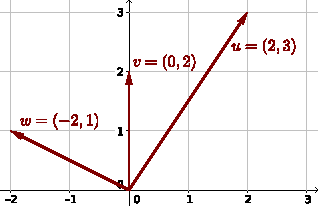
\includegraphics[width=7.0cm]{img/prova-3-nex-vetores-dom}
\end{center}
\begin{enumerate}
\item \textbf{(1,5)} Se $T$ é linear, qual das figuras abaixo \textbf{não} pode representar as imagens $T(u)$, $T(v)$ e $T(w)$? Justifique sua resposta exemplificando alguma propriedade das transformações lineares que não seria satisfeita.
\item \textbf{(1,5)} No caso da figura que é compatível com a definição de transformação linear, qual é a fórmula de $T(x,y)$?
\begin{multicols}{2}
\begin{itemize}
\item[] 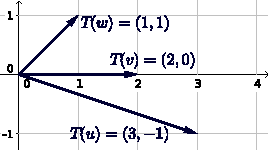
\includegraphics[width=6.4cm]{img/prova-3-nex-vetores-img1}
\item[] 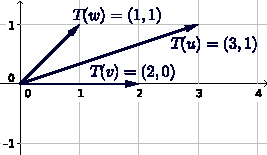
\includegraphics[width=6.4cm]{img/prova-3-nex-vetores-img2}
\end{itemize}
\end{multicols}
\end{enumerate}
\Answer
\begin{enumerate}
\item A segunda figura não mostra o seria obtido ao aplicar uma transformação linear à figura original pois, por exemplo, no domínio ocorre
\[
u = (2,3) = 2(0,2)-(-2,1) = 2v - w,
\]
enquanto que no contradomínio
\[
T(u) = (3,1) \neq (3,-1) = 2(2,0)-(1,1) = 2T(v) - T(w).
\]

\item Caso a primeira figura represente o resultado de aplicar uma transformação linear $T$ à figura original, pode-se obter a fórmula de $T$ usando a linearidade e os valores de $T$ nos vetores de qualquer base de $\R^2$. Por exemplo, considerando $B = \{ v, w \} = \{ (0,2), (-2,1) \}$, tem-se $(x,y) = \frac{2y+x}{4}(0,2) + \frac{-x}{2}(-2,1)$, para todo $(x,y) \in \R^2$. Logo,
\begin{align*}
T(x,y)
& = \frac{2y+x}{4}T(0,2) + \frac{-x}{2}T(-2,1)
  = \frac{2y+x}{4}(2,0) - \frac{x}{2}(1,1) \\
& = \left(\frac{2y+x}{2}, 0\right) - \left(\frac{x}{2}, \frac{x}{2}\right)
  = \left(y, -\frac{x}{2}\right).
\end{align*}
Esta fórmula é coerente com o que ocorre com o vetor $u$, pois
\[
T(u) = T(2,3) = \left(3,-\frac{2}{2}\right) = (3,-1).
\]
Assim, a primeira figura é compatível com a definição de transformação linear, e a fórmula da transformação linear correspondente é $T(x,y) = \left(y, -\frac{x}{2}\right)$.
\end{enumerate}

\end{ExerciseList}

\begin{center}
BOA PROVA!
\end{center}

\newpage
\restoregeometry
\section*{Respostas}
\shipoutAnswer
\end{document}
